\section{Runtime Application Tuning} \label{rat}

The Runtime Application Tuning (RAT) phase of READEX is carried out by the low-overhead READEX Runtime Library (RRL). RRL is implemented as a Score-P Substrate Plugin using the substrate plugin interface \cite{Schoene2017}. The plugin interface allows to utilize the instrumentation infrastructure of Score-P, without direct integration into Score-P. This approach reduces maintenance and integration efforts by keeping the RRL as a separate entity. As a substrate plugin, the RRL receives notifications for different events occurring during the application run via instrumentation, and uses this information to make switching decisions based on the application tuning model created at design-time.

The RRL implements three main mechanisms in order to apply the dynamic configuration switching at runtime, namely, scenario detection, configuration switching and calibration. The following sections detail the first two mechanisms, while Section~\ref{sec:calibration} describes the calibration mechanism, which is an extension to the standard version.

%\begin{figure}[!t]
%\centering
%%\includegraphics[trim={7cm 2cm 5.5cm 2cm},clip,width=3in]{readex-approach}
%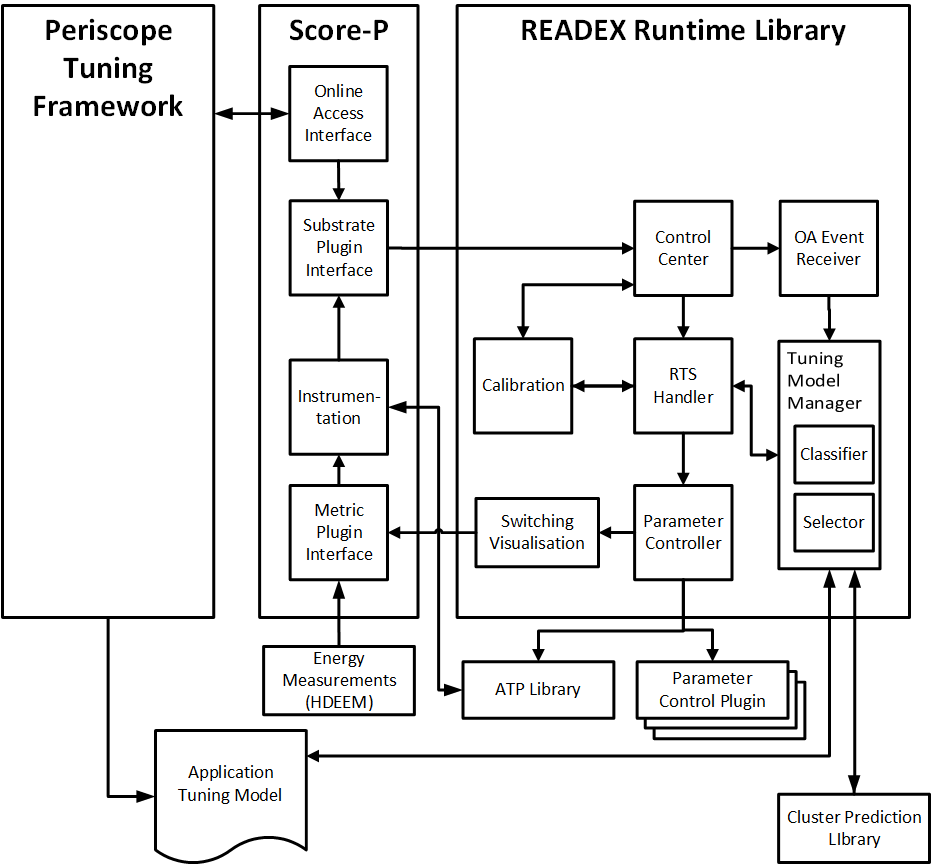
\includegraphics[width=.8\columnwidth]{figures/RRL_Architecture.png}
%\caption{Architecture of the READEX Runtime Library (RRL)}
%\label{fig:rrl}
%\end{figure}

\subsection{Scenario Detection}\label{scenario-detection}
Runtime detection of the upcoming scenario involves several steps. First, the ATM is loaded at the beginning of the application execution, and RRL reads the set of configurations, in the form of scenarios, classifiers and selectors. When a new application region is entered during the execution, RRL receives a notification of a region enter event from Score-P, and performs a check to detect if the encountered region is significant by searching for the region in the ATM. If the region is found, it is marked as a significant region. Otherwise, it is marked as an unknown region. 

Another check is performed to determine if the region must be tuned by computing the granularity of the region. The region will be tuned only if the granularity is above 100~ms. Once the region is determined to be both significant and coarse-granular enough, additional identifiers that are used to identify the current rts are requested. The current rts can then be identified by both the call stack and the additional identifiers. Finally, a new configuration is applied for the current rts to perform the configuration switching.
For an coarse-granular region marked as unknown, the calibration mechanism is invoked.

\subsection{Configuration Switching}\label{config-switching}
The scenario detection step applies a new configuration to the current region only if the region entered is found to be significant and coarse-granular. The setting for each tuning parameter is controlled by a dedicated Parameter Control Plugin (PCP). RRL performs the configuration switching by sending a request to the PCPs to set the new configuration. 

RRL supports two different modes for configuration switching: \textit{reset} and \textit{no-reset}. The \textit{reset} mode maintains a configuration stack. Whenever a new configuration is set, the previous configuration is pushed onto this stack. When the corresponding unset occurs, the element is removed from the stack and the previous configuration is set again. If the \textit{no-reset} mode is selected, the current configuration stays active until a new configuration is set, and the unset is ignored. This behaviour is configurable by the user. By default, the \textit{reset} mode is enabled.

\subsection{Calibration}\label{calibr}
READEX makes a distinction between seen and unseen rts's. For known or seen rts's that are already present in the ATM, RRL simply reads the optimal configuration, and performs configuration switching. For the unseen rts's, the RRL calibration mechanism, described in Section~\ref{sec:calibration} is used to find the optimal system configuration based on machine learning algorithms.

 
%Before the current region exits, the RTS Handler receives the notification  from Score-P through Control Center. The RTS Hander checks if the current region was set up for calibration. If yes, it requests the configuration for the currently exited region from the
%Calibration module. Once the RTS handler gets back the configuration from the calibration module, it passes this configuration to the TMM which stores the new configuration for the respective rts. If the region was not set up for calibration, then the Parameter Controller is informed that it might want to unset the current configuration. 

 